
\begin{frame}
	\frametitle{Warning Propagation Algorithm}
	Apply Message Passing to SAT
	\begin{itemize}
	\item Input: Formula in CNF and its Factor Graph
	\item Output: Valid variable assignment \newline
	      
	\end{itemize}
\end{frame}

\begin{frame}
	\frametitle{Warning Propagation Algorithm}
	Apply Message Passing to SAT
	\begin{itemize}
		\item Clause $a$ can send a \emph{warning} $u_{a\rightarrow i} \in \{0, 1\}$ to its variables $i$
		\item If $u_{a \rightarrow i} = 1$, $i$ \textbf{must} satisfy $a$ \newline e.g $\mathcal{F} = (\overline{x_1}) \land (x_1 \lor x_2)$ \newline$x_1$ has to satisfy the first clause
	
\begin{figure}[h]
\centering

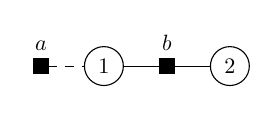
\begin{tikzpicture}[scale=0.8,transform shape]
   	\node[shape=circle,draw=black] (x1) at (1,0) {$1$};
    \node[shape=circle,draw=black] (x2) at (3,0) {$2$};
   
 

	\node[rectangle,draw=black, label = {$a$}, fill] (a) at (0,0) {};
	
	\node[rectangle,draw=black, label = {$b$}, fill] (b) at (2,0) {};

    \draw[-, >= stealth, dashed] (a) edge [right] node {} (x1);
 \draw[-, >= stealth] (b) edge [right] node {} (x1);
	 \draw[-, >= stealth] (b) edge [right] node {} (x2);

\end{tikzpicture}
%\caption{Subgraph of a factor tree with all messages required for computing $m_{a \rightarrow i}$}
\end{figure}
\item The clause $a$ \emph{fixes} the variable $i$ to the value $0$
\end{itemize}
\end{frame}

\begin{frame}
	\frametitle{Warning Propagation Algorithm}
	Apply Message Passing to SAT
	\begin{itemize}
		\item Variable $i$ receives warnings  $u_{b \rightarrow i}$
		\item $i$ to sends to $a$ its preferred value considering only the neighbours $b \neq a$
		\item \emph{Cavity Field} $h_{i \rightarrow a}$
		\begin{itemize}
		\item $>0$, if $i$ prefers the value $1$    \item $<0$ if $i$ prefers the value $0$
		\end{itemize}
		\item Messages
			\begin{itemize}
				\item Warnings $u_{a \rightarrow i} \in \{0, 1\}$
				\item Cavity Fields $h_{i \rightarrow a} \in \mathbb{Z}$
			\end{itemize}
	\end{itemize}
\end{frame}

\begin{frame}
	\frametitle{Update Rule - Cavity Field}
	
	\begin{itemize}
		\item Count how often $i$ is fixed to $1$ by clauses $b \neq a$
			$$ \sum_{b \in V_+(i) \setminus a} u_{b \rightarrow i}$$	
		\item Count how often $i$ is fixed to $0$ by clauses $b \neq a$
			$$ \sum_{b \in V_-(i) \setminus a} u_{b \rightarrow i}$$	
		\item Send the difference to $a$
			$$ h_{i \rightarrow a} = \sum_{b \in V_+(i) \setminus a} u_{b \rightarrow i} - \sum_{b \in V_-(i) \setminus a} u_{b \rightarrow i}$$
	\end{itemize}
\end{frame}

\begin{frame}
	\frametitle{Update Rule - Warnings}
	
	\begin{itemize}
		\item $a$ sends a warning to $i$, if its variables $j \neq i$ prefer to violate $a$
		\item Define $J_j^a = \begin{cases}
      -1, & \text{if } x_j = 1 \text{ satisfies a}  \\
      1, & \text{if } x_j = 0 \text{ satisfies a}
    \end{cases}$ 
    \item $j$ prefers to violate $a$, if $J_j^a h_{j \rightarrow a} > 0$ 
    \item Define $\theta(x) = \begin{cases}
      1, & x > 0  \\
      0, & x \leq 0
    \end{cases}$
	\end{itemize}
\end{frame}

\begin{frame}
	\frametitle{Update Rule - Warnings}
	
	\begin{itemize}
	\item $j$ prefers to violate $a$, if $J_j^a h_{j \rightarrow a} > 0$ 

    \item Define $\theta(x) = \begin{cases}
      1, & x > 0  \\
      0, & x \leq 0
    \end{cases}$
    
    \item Warnings can be computed as 
    $$u_{a \rightarrow i} = \prod_{j \in V(a) \setminus i} \theta(J_j^ah_{j\rightarrow a})$$
	\end{itemize}
\end{frame}

\begin{frame}
	\frametitle{Update Rule - Summary}
	$$ h_{i \rightarrow a} = \sum_{b \in V_+(i) \setminus a} u_{b \rightarrow i} - \sum_{b \in V_-(i) \setminus a} u_{b \rightarrow i}$$
	$$u_{a \rightarrow i} = \prod_{j \in V(a) \setminus i} \theta(J_j^ah_{j\rightarrow a})$$
\end{frame}
\begin{frame}
	\frametitle{Update Rule - Summary}
	$$ h_{i \rightarrow a} = - \sum_{b \in V_(i) \setminus a} J_i^b u_{b \rightarrow i}$$
	$$u_{a \rightarrow i} = \prod_{j \in V(a) \setminus i} \theta(J_j^ah_{j\rightarrow a})$$
\end{frame}

\begin{frame}
$$\mathcal{F} = \underbrace{\overline{x_1}}_{a} \land \underbrace{ x_5}_b \land \underbrace{(x_1 \lor \overline{x_2} \lor \overline{x_5})}_c \land  \underbrace{(x_2 \lor x_3 \lor x_4)}_d$$
\begin{figure}[h]
\centering

\begin{tikzpicture}[scale=1.0,transform shape]
	
   \node[rectangle,draw=black, label = left:{$a$}, fill] (a) at (0,1.5) {};
   \node[rectangle,draw=black, label = above:{$c$}, fill] (b) at (3,0) {};
  % \node[rectangle,draw=black, label = above:{$c$}, fill] (c) at (2,4) {};
   \node[rectangle,draw=black, label = below left:{$d$}, fill] (d) at (6,0) {};

   \node[rectangle,draw=black, label = left:{$b$}, fill] (e) at (0,-1.5) {};

   	
   	\node[shape=circle,draw=black, scale = 0.7] (x1) at (1.5,1.5) {$1$};
    \node[shape=circle,draw=black, scale = 0.7] (x2) at (4.5,0) {$2$};
    \node[shape=circle,draw=black, scale = 0.7] (x4) at (7,1) {$4$};
    \node[shape=circle,draw=black, scale = 0.7] (x3) at (7,-1) {$3$};
	   	\node[shape=circle,draw=black, scale = 0.7] (x5) at (1.5,-1.5) {$5$};


\draw[->, >= stealth, dashed] (a) edge [bend right, pos=0.5, below] node {\only<2-18>{1}} (x1);
\only<2>{\draw[->, >= stealth, thick ,dashed] (a) edge [bend right, pos=0.5, below] node {\only<2-20>{1}} (x1);}

\draw[<-, >= stealth, dashed] (a) edge [bend left, above] node {\only<17-17>{0}} (x1);
\only<17>{\draw[<-, >= stealth, dashed, thick] (a) edge [bend left, above] node {\only<1-17>{0}} (x1);}

	 
\draw[<-, >= stealth] (x1) edge [bend left, above] node {\only<14-18>{0}} (b);
\only<14>{\draw[<-, >= stealth, thick] (x1) edge [bend left, above] node {0} (b);}

\draw[->, >= stealth] (x1) edge [bend right, left] node[pos = 0.3] {\only<4-17>{-1}} (b);
\only<4>{\draw[->, >= stealth, thick] (x1) edge [bend right, left] node[pos = 0.3] {-1} (b);}

\draw[->, >= stealth, dashed] (b) edge [bend right, below] node {\only<6-18>{1}} (x2);
\only<6>{\draw[->, >= stealth, dashed, thick] (b) edge [bend right, below] node {\only<6-10>{1}} (x2);}

\draw[<-, >= stealth, dashed] (b) edge [bend left, above] node[pos = 0.5] {\only<13-17>{0}} (x2);
\only<13>{\draw[<-, >= stealth, dashed, thick] (b) edge [bend left, above] node[pos = 0.5] {0} (x2);}


%\draw[->, >= stealth] (x2) edge [bend right, right] node {\only<1-10>{x}} (c);
%\draw[<-, >= stealth] (x2) edge [bend left, left] node[pos = 0.8] {\only<1-10>{x}} (c);


\draw[->, >= stealth] (x2) edge [bend right, below] node[pos = 0.1] {\only<7-17>{-1}} (d);
\only<7>{\draw[->, >= stealth, thick] (x2) edge [bend right, below] node[pos = 0.1] {-1} (d);}

\draw[<-, >= stealth] (x2) edge [bend left, above] node[pos = 0.5] {\only<12-18>{0}} (d);
\only<12>{\draw[<-, >= stealth, thick] (x2) edge [bend left, above] node[pos = 0.5] {0} (d);}


\draw[->, >= stealth] (d) edge [bend right, below] node[pos = 0.8] {\only<10-18>{0}} (x4);
\only<10>{\draw[->, >= stealth, thick] (d) edge [bend right, below] node[pos = 0.8] {0} (x4);}

\draw[<-, >= stealth] (d) edge [bend left, above] node[pos = 0.7] {\only<8-17>{0}} (x4);
\only<8>{\draw[<-, >= stealth, thick] (d) edge [bend left, above] node[pos = 0.7] {\only<8-10>{0}} (x4);}


\draw[->, >= stealth] (d) edge [bend right, below] node[pos = 0.8] {\only<11-18>{0}} (x3);
\only<11>{\draw[->, >= stealth, thick] (d) edge [bend right, below] node[pos = 0.8] {0} (x3);}


\draw[<-, >= stealth] (d) edge [bend left, above] node[pos = 0.8] {\only<9-17>{0}} (x3);
\only<9>{\draw[<-, >= stealth, thick] (d) edge [bend left, above] node[pos = 0.8] {0} (x3);}

\draw[->, >= stealth] (e) edge [bend right, pos=0.5, below] node {\only<3-18>{1}} (x5);
\only<3>{\draw[->, >= stealth, thick] (e) edge [bend right, pos=0.5, below] node {1} (x5);}

\draw[<-, >= stealth] (e) edge [bend left, above] node {\only<16-17>{0}} (x5);
\only<16>{\draw[<-, >= stealth, thick] (e) edge [bend left, above] node {\only<16-18>{0}} (x5);}


\draw[<-, >= stealth, dashed] (x5) edge [bend left, above] node {\only<15-18>{0}} (b);
\only<15>{\draw[<-, >= stealth, dashed, thick] (x5) edge [bend left, above] node {0} (b);}

\draw[->, >= stealth, dashed] (x5) edge [bend right, right] node {\only<5-17>{1}} (b);
\only<5>{\draw[->, >= stealth, thick, dashed] (x5) edge [bend right, right] node {1} (b);}

\end{tikzpicture}
%\caption{Subgraph of a factor tree with all messages required for computing $m_{a \rightarrow i}$}
\end{figure}
\end{frame}

\begin{frame}
	\frametitle{Decimation Algorithm}
	
	\begin{itemize}
		\item If a variable is fixed to different values, $\mathcal{F}$ is not satisfiable
		\item If not, the warnings lead to a partial assignment:
			\begin{itemize}
				\item Assign each variable with active warnings the value it was fixed to
				\item If all warnings are $0$, assign a random value to a random variable
			\end{itemize}
		
	\end{itemize}
\end{frame}

\begin{frame}[containsverbatim]
	\frametitle{Message Passing}
	Warning Inspired Decimation Algorithm
	\begin{lstlisting}[mathescape = true, gobble=15, basicstyle=\ttfamily]
		1. While there are unassigned variables
		2.     Run the WP Algorithm
		3.     If WP does not converge
		          return UNCONVERGED
		4.     If at least one variable is fixed
		        to different values return UNSAT
		5.     Choose a partial assignment
		6.     Clean the graph
		7. Return the complete assignment
	\end{lstlisting}
\end{frame}

\begin{frame}
\frametitle{Example}
$$\mathcal{F} = \overline{x_1} \land x_5 \land (x_1 \lor \overline{x_2} \lor \overline{x_5}) \land  (x_2 \lor x_3 \lor x_4)$$
\begin{figure}[h]
\centering

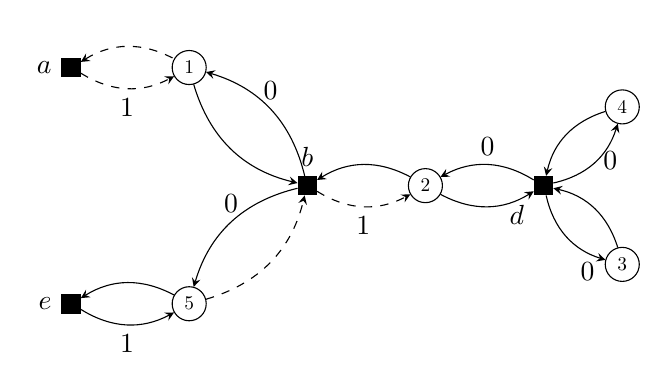
\begin{tikzpicture}[scale=1.0,transform shape]
	
   \node[rectangle,draw=black, label = left:{$a$}, fill] (a) at (0,1.5) {};
   \node[rectangle,draw=black, label = above:{$b$}, fill] (b) at (3,0) {};
  % \node[rectangle,draw=black, label = above:{$c$}, fill] (c) at (2,4) {};
   \node[rectangle,draw=black, label = below left:{$d$}, fill] (d) at (6,0) {};

   \node[rectangle,draw=black, label = left:{$e$}, fill] (e) at (0,-1.5) {};

   	
   	\node[shape=circle,draw=black, scale = 0.7] (x1) at (1.5,1.5) {$1$};
    \node[shape=circle,draw=black, scale = 0.7] (x2) at (4.5,0) {$2$};
    \node[shape=circle,draw=black, scale = 0.7] (x4) at (7,1) {$4$};
    \node[shape=circle,draw=black, scale = 0.7] (x3) at (7,-1) {$3$};
	   	\node[shape=circle,draw=black, scale = 0.7] (x5) at (1.5,-1.5) {$5$};


\draw[->, >= stealth, dashed] (a) edge [bend right, pos=0.5, below] node {1} (x1);


\draw[<-, >= stealth, dashed] (a) edge [bend left, above] node {} (x1);
	 
\draw[<-, >= stealth] (x1) edge [bend left, above] node {0} (b);

\draw[->, >= stealth] (x1) edge [bend right, left] node[pos = 0.3] {} (b);

\draw[->, >= stealth, dashed] (b) edge [bend right, below] node {1} (x2);

\draw[<-, >= stealth] (b) edge [bend left, above] node[pos = 0.5] {} (x2);

\draw[->, >= stealth] (x2) edge [bend right, below] node[pos = 0.1] {} (d);

\draw[<-, >= stealth] (x2) edge [bend left, above] node[pos = 0.5] {0} (d);

\draw[->, >= stealth] (d) edge [bend right, below] node[pos = 0.8] {0} (x4);

\draw[<-, >= stealth] (d) edge [bend left, above] node[pos = 0.7] {} (x4);

\draw[->, >= stealth] (d) edge [bend right, below] node[pos = 0.8] {0} (x3);

\draw[<-, >= stealth] (d) edge [bend left, above] node[pos = 0.8] {} (x3);

\draw[->, >= stealth] (e) edge [bend right, pos=0.5, below] node {1} (x5);

\draw[<-, >= stealth] (e) edge [bend left, above] node {} (x5);

\draw[<-, >= stealth] (x5) edge [bend left, above] node {0} (b);

\draw[->, >= stealth, dashed] (x5) edge [bend right, right] node {} (b);
\end{tikzpicture}
%\caption{Subgraph of a factor tree with all messages required for computing $m_{a \rightarrow i}$}
\end{figure}
Assign $x_1 = 0, \ x_2 = 0, \  x_5 = 1$

\end{frame}
\begin{frame}
\frametitle{Example}
\begin{itemize}
	\item Cleaned formula: $\mathcal{F} = (x_3 \lor x_4)$
	\item Cleaned graph:
	
\begin{figure}
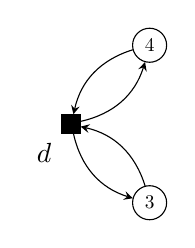
\begin{tikzpicture}[scale=1.0,transform shape]
	
   \node[rectangle,draw=black, label = below left:{$d$}, fill] (d) at (6,0) {};


   	
    \node[shape=circle,draw=black, scale = 0.7] (x4) at (7,1) {$4$};
    \node[shape=circle,draw=black, scale = 0.7] (x3) at (7,-1) {$3$};





\draw[->, >= stealth] (d) edge [bend right, below] node[pos = 0.8] {} (x4);

\draw[<-, >= stealth] (d) edge [bend left, above] node[pos = 0.7] {} (x4);

\draw[->, >= stealth] (d) edge [bend right, below] node[pos = 0.8] {} (x3);

\draw[<-, >= stealth] (d) edge [bend left, above] node[pos = 0.8] {} (x3);


\end{tikzpicture}

\end{figure}
\end{itemize}
\end{frame}